%CUT AND PASTE THIS ENTIRE DOCUMENT INTO A BLANK DOCUMENT ON CloudSageMath. Then replace the content (title, name, and so on), with your stuff. If you have problems or errors, let me know! 

%\documentclass[12pt]{amsart}
\documentclass{article}

\usepackage{tikz-cd}

%Python Code Listing
\usepackage[utf8]{inputenc}
\usepackage[english]{babel}
\usepackage[T1]{fontenc}

\usepackage{xcolor}
\definecolor{maroon}{cmyk}{0, 0.87, 0.68, 0.32}
\definecolor{halfgray}{gray}{0.55}
\definecolor{ipython_frame}{RGB}{207, 207, 207}
\definecolor{ipython_bg}{RGB}{247, 247, 247}
\definecolor{ipython_red}{RGB}{186, 33, 33}
\definecolor{ipython_green}{RGB}{0, 128, 0}
\definecolor{ipython_cyan}{RGB}{64, 128, 128}
\definecolor{ipython_purple}{RGB}{170, 34, 255}



\usepackage{listings}
\lstset{
    breaklines=true,
    %
    extendedchars=true,
    literate=
    {á}{{\'a}}1 {é}{{\'e}}1 {í}{{\'i}}1 {ó}{{\'o}}1 {ú}{{\'u}}1
    {Á}{{\'A}}1 {É}{{\'E}}1 {Í}{{\'I}}1 {Ó}{{\'O}}1 {Ú}{{\'U}}1
    {à}{{\`a}}1 {è}{{\`e}}1 {ì}{{\`i}}1 {ò}{{\`o}}1 {ù}{{\`u}}1
    {À}{{\`A}}1 {È}{{\'E}}1 {Ì}{{\`I}}1 {Ò}{{\`O}}1 {Ù}{{\`U}}1
    {ä}{{\"a}}1 {ë}{{\"e}}1 {ï}{{\"i}}1 {ö}{{\"o}}1 {ü}{{\"u}}1
    {Ä}{{\"A}}1 {Ë}{{\"E}}1 {Ï}{{\"I}}1 {Ö}{{\"O}}1 {Ü}{{\"U}}1
    {â}{{\^a}}1 {ê}{{\^e}}1 {î}{{\^i}}1 {ô}{{\^o}}1 {û}{{\^u}}1
    {Â}{{\^A}}1 {Ê}{{\^E}}1 {Î}{{\^I}}1 {Ô}{{\^O}}1 {Û}{{\^U}}1
    {œ}{{\oe}}1 {Œ}{{\OE}}1 {æ}{{\ae}}1 {Æ}{{\AE}}1 {ß}{{\ss}}1
    {ç}{{\c c}}1 {Ç}{{\c C}}1 {ø}{{\o}}1 {å}{{\r a}}1 {Å}{{\r A}}1
    {€}{{\EUR}}1 {£}{{\pounds}}1
}

%%
%% Python definition (c) 1998 Michael Weber
%% Additional definitions (2013) Alexis Dimitriadis
%% modified by me (should not have empty lines)
%%
\lstdefinelanguage{iPython}{
    morekeywords={access,and,break,class,continue,def,del,elif,else,except,exec,finally,for,from,global,if,import,in,is,lambda,not,or,pass,print,raise,return,try,while},%
    %
    % Built-ins
    morekeywords=[2]{abs,all,any,basestring,bin,bool,bytearray,callable,chr,classmethod,cmp,compile,complex,delattr,dict,dir,divmod,enumerate,eval,execfile,file,filter,float,format,frozenset,getattr,globals,hasattr,hash,help,hex,id,input,int,isinstance,issubclass,iter,len,list,locals,long,map,max,memoryview,min,next,object,oct,open,ord,pow,property,range,raw_input,reduce,reload,repr,reversed,round,set,setattr,slice,sorted,staticmethod,str,sum,super,tuple,type,unichr,unicode,vars,xrange,zip,apply,buffer,coerce,intern},%
    %
    sensitive=true,%
    morecomment=[l]\#,%
    morestring=[b]',%
    morestring=[b]",%
    %
    morestring=[s]{'''}{'''},% used for documentation text (mulitiline strings)
    morestring=[s]{"""}{"""},% added by Philipp Matthias Hahn
    %
    morestring=[s]{r'}{'},% `raw' strings
    morestring=[s]{r"}{"},%
    morestring=[s]{r'''}{'''},%
    morestring=[s]{r"""}{"""},%
    morestring=[s]{u'}{'},% unicode strings
    morestring=[s]{u"}{"},%
    morestring=[s]{u'''}{'''},%
    morestring=[s]{u"""}{"""},%
    %
    % {replace}{replacement}{lenght of replace}
    % *{-}{-}{1} will not replace in comments and so on
    literate=
    {á}{{\'a}}1 {é}{{\'e}}1 {í}{{\'i}}1 {ó}{{\'o}}1 {ú}{{\'u}}1
    {Á}{{\'A}}1 {É}{{\'E}}1 {Í}{{\'I}}1 {Ó}{{\'O}}1 {Ú}{{\'U}}1
    {à}{{\`a}}1 {è}{{\`e}}1 {ì}{{\`i}}1 {ò}{{\`o}}1 {ù}{{\`u}}1
    {À}{{\`A}}1 {È}{{\'E}}1 {Ì}{{\`I}}1 {Ò}{{\`O}}1 {Ù}{{\`U}}1
    {ä}{{\"a}}1 {ë}{{\"e}}1 {ï}{{\"i}}1 {ö}{{\"o}}1 {ü}{{\"u}}1
    {Ä}{{\"A}}1 {Ë}{{\"E}}1 {Ï}{{\"I}}1 {Ö}{{\"O}}1 {Ü}{{\"U}}1
    {â}{{\^a}}1 {ê}{{\^e}}1 {î}{{\^i}}1 {ô}{{\^o}}1 {û}{{\^u}}1
    {Â}{{\^A}}1 {Ê}{{\^E}}1 {Î}{{\^I}}1 {Ô}{{\^O}}1 {Û}{{\^U}}1
    {œ}{{\oe}}1 {Œ}{{\OE}}1 {æ}{{\ae}}1 {Æ}{{\AE}}1 {ß}{{\ss}}1
    {ç}{{\c c}}1 {Ç}{{\c C}}1 {ø}{{\o}}1 {å}{{\r a}}1 {Å}{{\r A}}1
    {€}{{\EUR}}1 {£}{{\pounds}}1
    %
    {^}{{{\color{ipython_purple}\^{}}}}1
    {=}{{{\color{ipython_purple}=}}}1
    %
    {+}{{{\color{ipython_purple}+}}}1
    {*}{{{\color{ipython_purple}$^\ast$}}}1
    {/}{{{\color{ipython_purple}/}}}1
    %
    {+=}{{{+=}}}1
    {-=}{{{-=}}}1
    {*=}{{{$^\ast$=}}}1
    {/=}{{{/=}}}1,
    literate=
    *{-}{{{\color{ipython_purple}-}}}1
     {?}{{{\color{ipython_purple}?}}}1,
    %
    identifierstyle=\color{black}\ttfamily,
    commentstyle=\color{ipython_cyan}\ttfamily,
    stringstyle=\color{ipython_red}\ttfamily,
    keepspaces=true,
    showspaces=false,
    showstringspaces=false,
    %
    rulecolor=\color{ipython_frame},
    frame=single,
    frameround={t}{t}{t}{t},
    framexleftmargin=6mm,
    numbers=left,
    numberstyle=\tiny\color{halfgray},
    %
    %
    backgroundcolor=\color{ipython_bg},
    %   extendedchars=true,
    basicstyle=\scriptsize,
    keywordstyle=\color{ipython_green}\ttfamily,
}

%%%%flowchart
\usetikzlibrary{shapes.geometric, arrows}
\tikzstyle{startstop} = [rectangle, rounded corners, minimum width=3cm, minimum height=1cm, text width=25em,text centered, draw=black, fill=yellow!30]
\tikzstyle{io} = [trapezium, trapezium left angle=70, trapezium right angle=110, minimum width=3cm, minimum height=1cm, text centered, draw=black, fill=blue!30]
\tikzstyle{process} = [rectangle, minimum width=3cm, minimum height=1cm, text width=15em, text centered, draw=black, fill=orange!30]
%\tikzstyle{decision} = [diamond, minimum width=3cm, minimum height=1cm, text centered, draw=black, fill=green!30]
\tikzstyle{arrow} = [thick,->,>=stealth]

\tikzstyle{decision} = [rectangle, rounded corners, draw, fill=blue!20, 
    text width=15em, text badly centered, node distance=2.2cm, inner sep=0pt]
\tikzstyle{block} = [rectangle, draw, fill=blue!20, 
    text width=5em, text centered, rounded corners, minimum height=4em]
\tikzstyle{line} = [draw, -latex']
\tikzstyle{cloud} = [draw, ellipse,fill=red!20, node distance=3cm,
    minimum height=2em]
%\usepackage[english]{babel}
%\usepackage[utf8]{inputenc}
%\usepackage[margin=1in]{geometry}
%\usepackage[titletoc,title]{appendix}
\usepackage{array}
\usepackage{amsmath,amsfonts,amssymb,mathtools}
\usepackage{amsthm}
%These commands deal with theorem-like environments (i.e., italic)
\theoremstyle{plain}
%\newtheorem{theorem}{Theorem}
%\newtheorem{proposition}{Proposition}
%\newtheorem{corollary}{Corollary}
\newtheorem{property}{Property}
%\newtheorem{definition}{Definition}
%\newtheorem{proof}{Proof}
%\newtheorem{lemma}{Lemma}
%\newtheorem{claim}{Claim}
%\newtheorem{example}{Example}
\newtheorem{non-example}{Non-Example}

\DeclareMathOperator{\id}{id}
\DeclareMathOperator{\Tr}{Tr}


\usepackage{hyperref}

\usepackage{graphicx}
\usepackage{tikz,lipsum,lmodern}
\usepackage[most]{tcolorbox}

%\thispagestyle{empty}

%%%%%%from math 729

\usepackage[]{algorithm2e}
\usepackage{graphicx,float}
\usepackage{tikz}
\usetikzlibrary{graphs,graphs.standard,quotes}
\usepackage{multicol}
\usepackage{capt-of}

\usepackage{amscd,amsthm,amsmath,amssymb,amsfonts,latexsym,
graphicx,enumerate,setspace,verbatim,tocloft,rotating}
%\usepackage{color}                    % For creating colored text and background
%\usepackage{hyperref}                 % For creating hyperlinks in cross references
% other possibly useful packages: textcomp,mathrsfs,amscd,epsfig,euscript,cancel

%%%%% Layout
% These numbers might depend on your printer. Check the margins and compare them to the Graduate Division's
% guidelines. If there's something off, try playing with the numbers...
%
% For chapters:
%     Must have a minimum of 1.5in margin on left and 1in on all other sides.  Where there are page numbers
%     (whether on top or bottom), must have one additional inch between the page number and the text, for a
%     total of 2in between the edge of the paper and the text.
% For frontmatter pages:
%     The same margin numbers generally work, except for the Title Page, so you will notice that we use
%     some numbers for \textheight and \footskip right here, and then change them below, right after
%     generating the Title Page.

\hoffset=.5in 
\oddsidemargin=0in   % = 1in because LaTeX adds 1in
\evensidemargin=0in  % = 1in because LaTeX adds 1in
\topmargin=0in       % = 1in because LaTeX adds 1in
\headheight=0in
\headsep=1in         % Distance from top of pagenum (for page numbers at top-right corner of page) to text
\footskip=1.2in      % Distance from bottom of text to the page number (for page number at bottom of page)
\textwidth=5.9in     % Should be 6in, but use 5.9in to be conservative
\textheight=8.0in    % Best for Title Page (will change after the Title Page)

\pagestyle{plain}

\doublespacing

%%%%% Style of theorems, definitions, examples, equations, etc.

\theoremstyle{plain} % Heading is bold, text italic.
%\newtheorem{theorem}{Theorem}[chapter]
%\newtheorem{lemma}[theorem]{Lemma}
\newtheorem{proposition}{Proposition}
%\newtheorem{corollary}[theorem]{Corollary}
%\newtheorem{conjecture}{Conjecture}[chapter]
\newtheorem*{utheorem}{Theorem}
\newtheorem*{ucorollary}{Corollary}
\newtheorem{theorem}{Theorem}
\newtheorem{lemma}{Lemma}
\newtheorem*{ulemma}{Lemma}
\newtheorem{definition}[theorem]{Definition}

\theoremstyle{definition}  % Heading is bold, text is roman
%\newtheorem{definition}{Definition}[chapter]
%\newtheorem{example}{Example}[chapter]

\theoremstyle{remark}  % Heading is italic, text is roman
\newtheorem*{remark}{Remark}
\newtheorem*{note}{Note}
%\newtheorem{claim}{Claim}[chapter]

% Shortcuts (add your own...):
\newcommand{\N}{\mathbb{N}}
\newcommand{\Z}{\mathbb{Z}}
\newcommand{\Q}{\mathbb{Q}}
\newcommand{\R}{\mathbb{R}}
\newcommand{\C}{\mathbb{C}}
\newcommand{\e}[1]{{\mathbb E}\left[ #1 \right]}


%%%%flowchart
\usetikzlibrary{shapes.geometric, arrows}
\tikzstyle{startstop} = [rectangle, rounded corners, minimum width=3cm, minimum height=1cm, text width=25em,text centered, draw=black, fill=yellow!30]
\tikzstyle{io} = [trapezium, trapezium left angle=70, trapezium right angle=110, minimum width=3cm, minimum height=1cm, text centered, draw=black, fill=blue!30]
\tikzstyle{process} = [rectangle, minimum width=3cm, minimum height=1cm, text width=15em, text centered, draw=black, fill=orange!30]
%\tikzstyle{decision} = [diamond, minimum width=3cm, minimum height=1cm, text centered, draw=black, fill=green!30]
\tikzstyle{arrow} = [thick,->,>=stealth]

\tikzstyle{decision} = [rectangle, rounded corners, draw, fill=blue!20, 
    text width=15em, text badly centered, node distance=2.2cm, inner sep=0pt]
\tikzstyle{block} = [rectangle, draw, fill=blue!20, 
    text width=5em, text centered, rounded corners, minimum height=4em]
\tikzstyle{line} = [draw, -latex']
\tikzstyle{cloud} = [draw, ellipse,fill=red!20, node distance=3cm,
    minimum height=2em]
%\usepackage[english]{babel}
%\usepackage[utf8]{inputenc}
%\usepackage[margin=1in]{geometry}
%\usepackage[titletoc,title]{appendix}
\usepackage{array}
\usepackage{amsmath,amsfonts,amssymb,mathtools}
\usepackage{amsthm}
%These commands deal with theorem-like environments (i.e., italic)
\theoremstyle{plain}


%\DeclarePairedDelimiter\ceil{\lceil}{\rceil}
%\DeclarePairedDelimiter\floor{\lfloor}{\rfloor}

%%%%% Appendix style

\renewcommand\appendix[1]{
\chapter*{#1}
\addcontentsline{toc}{chapter}{#1}
}


\begin{document}

\title{The scaling factor in self-attention}

\author{William Chuang}

\maketitle

%\begin{tcolorbox}[enhanced,fit to height=10cm,
%  colback=green!25!black!10!white,colframe=green!75!black,title=Section 3.2.1 in 1706.03762,
%  drop fuzzy shadow,watermark color=white]
%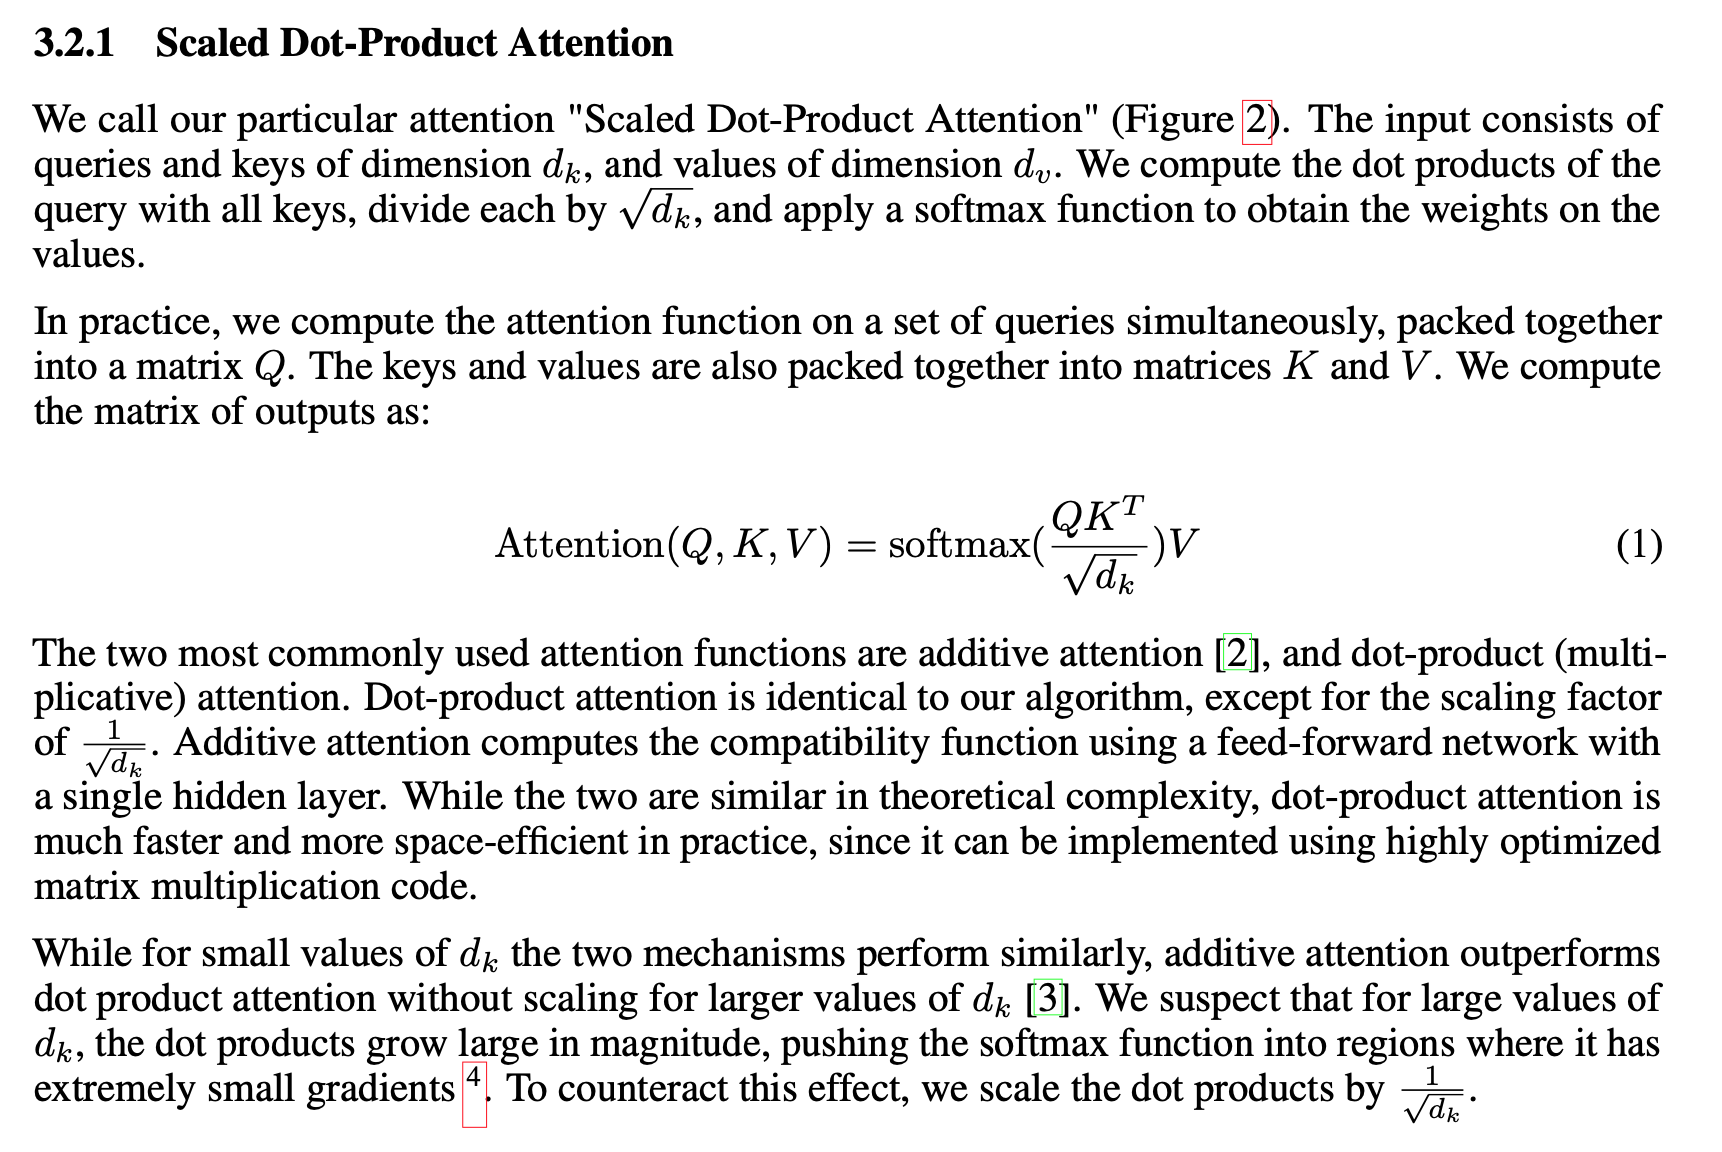
\includegraphics[scale=0.4]{1.png}
%\end{tcolorbox}

\section{Introduction}
In the context of deep learning neural networks, attention algorithms are designed for determining connections by weights between two elements in a sequential inputs. Self-attention was proposed by Vaswani et. al.\cite{vaswani2017attention} in 2017. Suppose a sequential input $X\in \mathbb{R}^N\times \mathbb{R}^{d_x}$ is given. Let $Q:=XW_q\in \mathbb{R}^{N}\times\mathbb{R}^{d_q}, K:=XW_k\in \mathbb{R}^{N}\times\mathbb{R}^{d_k}$, and $V:=XW_v\in \mathbb{R}^{N}\times\mathbb{R}^{d_v}$ where $W_k, W_v,$ and $W_q$ are initiated such that (i) $W_q\in\mathbb{R}^{d_x}\times\mathbb{R}^{d_q}$, $W_k\in\mathbb{R}^{d_x}\times\mathbb{R}^{d_k}$, and $W_v\in\mathbb{R}^{d_x} \times \mathbb{R}^{d_v}$, (ii) the variance of the inner product of each row vector in $X$ with each column vector in either $W_q, W_k,$ or $W_v$ to be unit, (iii) each row vector in $Q$ denoted by $q_i$, and each row vector in $K$ denoted by $k_i$ to be random variables with zero means, i.e. $\mathbb{E} q_i=0=\mathbb{E} k_i, \forall i$, and unit variances, i.e $\text{Var} q_i=1=\text{Var}k_i$, where $i\in\left\lbrace 1,...,d_k\right\rbrace$, and (iv) $q_i$ and $k_j$ are all independent in the following ways: $\text{Cov}\left( q_i,k_i\right)=0, \forall i,$ $\text{Cov}\left( q_i,q_j\right)=0, \forall i\neq j, \text{ and}$ $\text{Cov}\left( k_i,k_j\right)=0, \forall i\neq j.$ By convention, let $d_k=d_q$. Then the each scalar product of column vectors in $Q$ and $K$ has variance $d_k$ (see Appendix).
 
\begin{definition}[Self-attention]
The self-attention is the following function
$$
\text{Attention}\left(Q,K,V\right):= \left( \text{softmax}\left(\frac{\left( QK^T \right)_i}{\sqrt{d_k}} \right)_{i=1}^N \right)_{N \times N} \circ V_{N \times d_v}.
$$

\end{definition}
\noindent\textbf{Remark:} The Softmax function is defined using the Boltzmann distribution function: Given a finite sequence $\left\lbrace z_i\right\rbrace, j\in\left\lbrace 1,...,n\right\rbrace$, then 
$$
\text{Softmax}(z_i) := \frac{\exp\left(z_i \right) }{\sum\limits_j \exp\left(z_j \right)}.
$$

Since the sum of the above function adds up to one, i.e. $\sum\limits_{i=1}^n \text{Softmax}(z_i) =1$, it is a probability distribution. In physics, this distribution is called Boltzmann distribution. Furthermore, this distribution can be scaled by using a parameter $\beta$, and $\beta$ is the inverse of the temperature of the physical system described by the distribution:
$$
\text{Softmax}(\beta z_i) := \frac{\exp\left(\beta z_i \right) }{\sum\limits_j \exp\left(\beta z_j \right)}.
$$

In self-attention, this $\beta$ is $\frac{1}{\sqrt{d_k}}$, and $T$ is the standard deviation of the scalar product $\sqrt{d_k}$.

Apply Softmax to column vectors in the matrix $\frac{QK^T}{\sqrt{d_k}}$, meaning each entry of the matrix $\text{softmax}\left(\frac{QK^T}{\sqrt{d_k}} \right)_{N\times N}$ is obtained by taking the scalar product on the $i$-th row of $Q$ to multiply the $j-th$ column of $K^T$, then divide the scalar product by $\sqrt{d_k}$, and then apply Softmax function on each column of the matrix $\left(\frac{QK^T}{\sqrt{d_k}}\right)_{N\times N}$. Finally, take matrix multiplication between $\text{softmax}\left(\frac{QK^T}{\sqrt{d_k}} \right)_{N\times N}$ and $V_{N \times d_v}$. 

Hence, in self-attention, each attention, i.e. weight, between each element in the sequential input to the other element in the same sequential input was weighted by the Boltzmann distribution $\text{softmax}\left(\frac{\left( QK^T \right)_i}{\sqrt{d_k}} \right)_{i=1}^N$.

Furthermore, because of the random initiation of each weight matrices, if this self-attention, i.e. weights assigning process were run in parallel, then the model can learn from more than one different perspectives. In \cite{vaswani2017attention}, this notion is defined as multi-head attention. Each self-attention function  $\text{Attention}\left(Q,K,V\right)_i$ is called $\text{head}_i$, where $i$ is from 1 to $H$. The output of all $H$ heads are concatenated to a tensor denoted by $\text{Concat}\left(\text{head}_1,...,\text{head}_H \right)$, then defined $\text{Multihead(Q,K,V)}:= \text{Concat}\left(\text{head}_1,...,\text{head}_H \right)\circ W^O$, where $W^O\in \mathbb{R}^{H\cdot d_v}\times \mathbb{R}^{d_{\text{out}}}$.


Let $\epsilon>0$ be given. Because of the mathematical form of the Boltzmann distribution, if the input is $z_i+\epsilon$, then $\text{Softmax}(\beta z_i+\epsilon)=\text{Softmax}(\beta z_i).$ However, a naive but natural question to ask is what if the scaling factor $\beta$ in Boltzmann distribution, or the self-attention function, is modified into the form $\beta^\epsilon$ or $\beta\cdot\epsilon$? It is necessary to ask this question, since we want to be able to justify why and when it makes sense to use the scaling factor $\beta=\frac{1}{\sqrt{d_k}}$ in the self-attention function. Is it sufficient to ask this question? That is the question this paper is going to answer. The next section provides a solution to this question.


\section{Algorithm}

To be able to make sense to use the scaling factor $\beta=\frac{1}{\sqrt{d_k}}$ in self-attention function, the four assumptions are necessary. 

Within the four assumptions, the first assumption is usually fixed when self-attention is considered to be applied. 


Since the way query and key matrices are defined, i.e. $Q=XW_q$ and $K=XW_k$, assumption (iii) and (iv) are based on assumption (ii).

Suppose the assumptions (ii) is relaxed, the variance of the scalar product $q_ik_i$ is approximated to $\left( d_x \sigma_X^2 \sigma_{W_q}^2\right)\cdot\left(d_x \sigma_X^2 \sigma_{W_k}^2\right)\cdot d_k$. Since the training set is given, i.e. it is fixed, and so are $d_x$ and $d_k$, $\sigma_{W_q}$ and $\sigma_{W_k}$ are the actual moving factors. 

What can cause $\sigma_{W_q}$ and $\sigma_{W_k}$ to be changed? In the training phase, the gradient descent algorithm or the backpropagation is used and the algorithm is going to shift the initial probability distribution of each entry in the random matrices $W_q$ and $W_k$ to the final probability distribution at a local minimum in the moduli space (or on the loss surface).

Hence, the scaling factor $\beta=\frac{1}{\sqrt{d_k}}$ is only valid at the initial point given the four assumptions at the initial point in the moduli space, and it can hold true if the thermodynamic system described by the Boltzmann distribution is in statics, i.e. its temperature is fixed. However, since the initial point is random and unlikely to be the final point in the moduli space throughout the training mode, the assumption (ii) is not valid right after the training of the model that used self-attention function is initiated. Without assumption (ii), assumption (iii) and (iv) are invalid throughout the training and predicting modes.


To solve this problem, the solution could be written as an algorithm that it measures $\sigma_{W_q}$ and $\sigma_{W_k}$ and updates the scaling factor $\beta$ in after each iteration or batch during the training and the best scaling factor $\beta$ that is going to be used in the predicting mode could be determined by the best model chosen from the ensemble of all trained models.

This also answers the question asked in the previous section that it shows the sufficiency to ask the question.





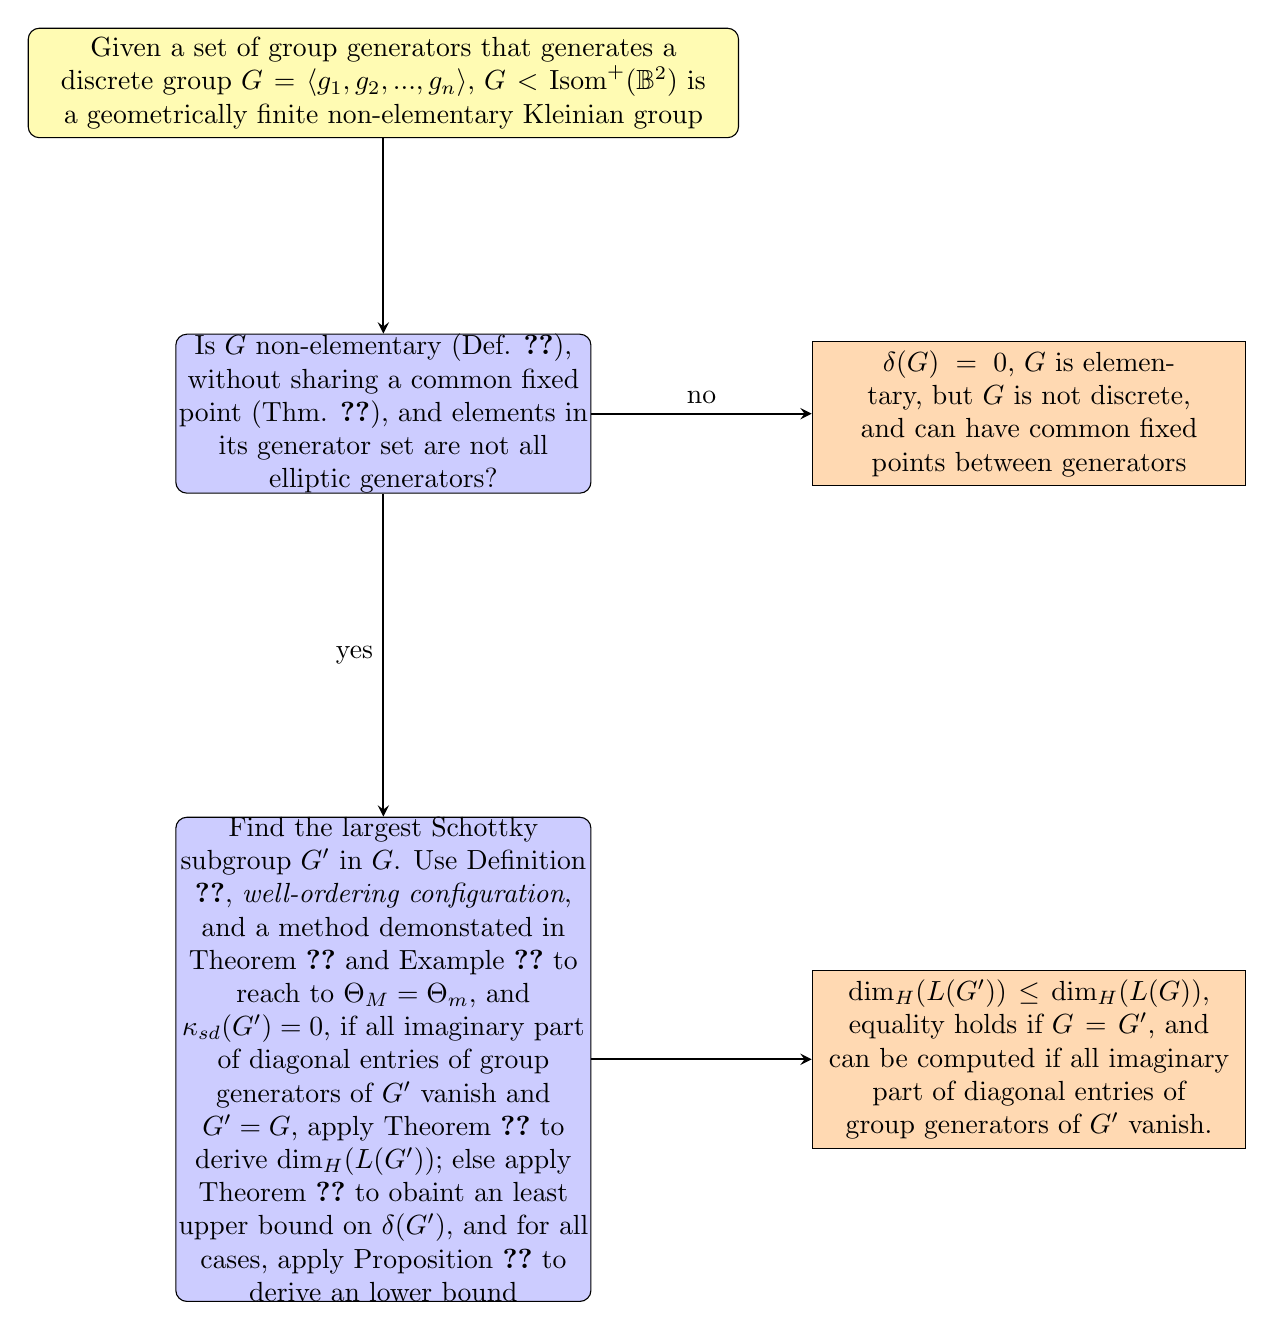
\begin{tikzpicture}[node distance=0.2cm]
\node (start) [startstop] {Given a set of group generators that generates a discrete group $G=\left\langle g_1,g_2,...,g_n\right\rangle$, $G<\text{Isom}^+(\mathbb{B}^2)$ is a geometrically finite non-elementary Kleinian group};
%\node (dec2) [decision, below of=start] {Is $G$ discrete?};
%\node (stop2) [process, right of=dec2, xshift=8cm] {$\nexists \delta(G)$};


\node (dec3) [decision, below of=start, yshift=-2cm] {Is $G$ non-elementary (Def. \ref{elementary}), without sharing a common fixed point (Thm. \ref{Theorem 5.3.3 ratcliffe}), and elements in its generator set are not all elliptic generators?};
%\node (dec7) [decision, below of=dec3, yshift=-2cm] {Does $G$ have elliptic generators?};

\node (stop3) [process, right of=dec3, xshift=8cm] {$\delta(G)=0$, $G$ is elementary, but $G$ is not discrete, and can have common fixed points between generators};
\node (dec4) [decision, below of=dec3, yshift=-6cm] {Find the largest Schottky subgroup $G'$ in $G$. Use Definition \ref{spacing difference}, \textit{well-ordering configuration}, and a method demonstated in Theorem \ref{main thm 2} and Example \ref{main thm 2 ex} to reach to $\Theta_M=\Theta_m$, and $\kappa_{sd}(G')=0$, if all imaginary part of diagonal entries of group generators of $G'$ vanish and $G'=G$, apply Theorem \ref{main thm 11} to derive $\dim_{H}(L(G'))$; else apply Theorem \ref{main thm 10} to obaint an least upper bound on $\delta(G')$, and for all cases, apply Proposition \ref{prop 1} to derive an lower bound};

\node (dec6) [process, right of=dec4, xshift=8cm] {$\dim_H(L(G'))\leq \dim_H(L(G))$, equality holds if $G=G'$, and can be computed if all imaginary part of diagonal entries of group generators of $G'$ vanish.};

%\node (pro3) [process, below of=dec4, yshift=-6cm] {use helper algorithm to find $\delta(G')$ as a lower bound, then use Abscissa convergence of $\mathcal{P}(G,t)$ to do a statistical estimation on $\delta(G)$; Thm. \ref{Theorem14.14inBorthwick} does not apply};

\draw [arrow] (start) -- (dec3);
%\draw [arrow] (dec1) -- node[anchor=south] {no}(stop1);
%\draw [arrow] (dec1) -- node[anchor=east] {yes}(dec2);
%\draw [arrow] (dec2) -- node[anchor=south] {no}(stop2);
\draw [arrow] (dec4) -- node[anchor=east] {}(dec6);
\draw [arrow] (dec3) -- node[anchor=south] {no}(stop3);
\draw [arrow] (dec3) -- node[anchor=east] {yes}(dec4);
%\draw [arrow] (dec7) -- node[anchor=east] {no}(dec4);


%\draw [arrow] (dec6) -- node[anchor=east] {no}(pro3);
%\draw [arrow] (dec6) -- node[anchor=south] {yes}(pro2);
%\draw [arrow] (dec4) --  node[anchor=west, below=2pt ] {no} ++(3.5,0) |- (dec6);
%\draw [arrow] (dec4.west) -|node[anchor=south]{no}++(-1,0)|- (dec6.west);
%\draw [arrow] (dec7.west) -|node[anchor=south]{yes}++(-2,0)|- (pro3.west);
%\path[line] (dec4) |- ([xshift=-0.5cm,yshift=-0.5cm]j.south west) |- (dec6);
%\draw [arrow] (dec4.west) -- ++ (5em,0) node[above] {no}-- ++(5em,0) |- (dec6.west);
\end{tikzpicture}

\section{Empirical examples}
\section{Discussion}
\section{Conclusion}
%\section{Limitation}

\section{Appendix: Deriving the scaling factor $\frac{1}{\sqrt{d_k}}$ used in \cite{vaswani2017attention}}

Let $X$ and $Y$ be random variables.

Firstly, recall the definition of variance\cite{folland1999real}:
\begin{definition}
$$
\sigma^2(X):=\inf\limits_{a\in\mathbb{R}}\mathbb{E}\left[\left(X-a \right)^2 \right].
$$
\end{definition}
Hence if $X\notin L^2$, then $\text{Var}[X]=\infty$. If $X\in L^2$, then $\mathbb{E}\left[\left(X-a \right)^2 \right]=\mathbb{E}(X^2)-2a\mathbb{E}(X)+a^2$ has a minimum at $a=\mathbb{E}(X)$, and the expression of the variance of $X$ can be rewritten using the minimum:
$$
\text{Var}[X]=\mathbb{E}\left[\left(X-a \right)^2 \right]=\mathbb{E}\left[\left(X- \mathbb{E}[X]\right)^2 \right].
$$
\begin{proposition}
$$
\text{Var}[X]=\mathbb{E}(X^2)+(\mathbb{E}[X])^2-2(\mathbb{E}[x])^2=\mathbb{E}(X^2)-(\mathbb{E}X)^2.
$$
\end{proposition}
\begin{proof}
$$
\text{Var}[X]=\mathbb{E}\left[X^2+\left( \mathbb{E} X\right)^2 -2X\mathbb{E}X\right]
$$
$$
=\mathbb{E}(X^2)+(\mathbb{E}[X])^2-2(\mathbb{E}[x])^2=\mathbb{E}(X^2)-(\mathbb{E}X)^2.
$$
\end{proof}
Secondly, 
\begin{definition}
the covariance of $X$ and $Y$ is:
$$
\text{Cov}[X,Y]:=\mathbb{E}\left[(X-\mathbb{E} X)(Y-\mathbb{E} Y) \right].
$$
\end{definition}
\begin{proposition}
$$
\text{Cov}[X,Y]=\mathbb{E}XY-\mathbb{E}X\mathbb{E}Y.
$$
\end{proposition}

\begin{proof}
$$
\text{Cov}[X,Y]=\mathbb{E} \left[ XY -X\mathbb{E} Y -Y\mathbb{E}X +\mathbb{E}X \mathbb{E}Y\right]
$$
$$
=\mathbb{E}XY-\mathbb{E}X\mathbb{E}Y-\mathbb{E}X\mathbb{E}Y+\mathbb{E}X\mathbb{E}Y
$$
$$
=\mathbb{E}XY-\mathbb{E}X\mathbb{E}Y.
$$
\end{proof}

Then, the expectation value of $X^2Y^2$ can be written in the following expression:
$$
\mathbb{E}X^2Y^2=\text{Cov}[X^2,Y^2]+\mathbb{E}X^2\mathbb{E}Y^2
$$
$$
=\text{Cov}[X^2,Y^2]+(\text{Var}X+(\mathbb{E} X)^2)(\text{Var}Y+(\mathbb{E} Y)^2).
$$

\begin{proposition}
If $X$ and $Y$ are independent and both have zero means, then 
$$
\text{Var}[XY]=\text{Var}X \text{Var}Y.
$$
\end{proposition}
\begin{proof}
By applying the above results, the variance of the product of $X$ and $Y$ can be derived:
$$
\text{Var}[XY]=\mathbb{E}X^2Y^2-(\mathbb{E}XY)^2
$$
$$
=\mathbb{E}X^2Y^2-(\mathbb{E}Y\mathbb{E}X+\text{Cov}[X,Y])^2
$$
$$
=\text{Cov}[X^2,Y^2]+(\text{Var}X+(\mathbb{E} X)^2)(\text{Var}Y+(\mathbb{E} Y)^2)-(\mathbb{E}Y\mathbb{E}X+\text{Cov}[X,Y])^2.
$$
Since $X$ and $Y$ are independent, then $\text{Cov}[X^2,Y^2]=0$, and 
$$
\text{Var}[XY]=(\text{Var}X+(\mathbb{E} X)^2)(\text{Var}Y+(\mathbb{E} Y)^2)-(\mathbb{E}Y\mathbb{E}X+\text{Cov}[X,Y])^2.
$$
Since $X$ and $Y$ are independent and both have zero means, i.e. $\mathbb{E}X=0=\mathbb{E}Y$, then
$$
\text{Var}[XY]=\text{Var}X \text{Var}Y.
$$
\end{proof}
\begin{proposition}
Let $X_i, i\in\left\lbrace 1,...,n\right\rbrace$ be $n$ independent variables. 
$$
\text{Var}\left( \sum\limits_{i} X_i\right)=\sum\limits_i \text{Var}X_i.
$$
\end{proposition}
\begin{proof}
Then 
$$
\text{Var}\left( \sum\limits_{i} X_i\right)=\mathbb{E} \left(\left( \sum\limits_{i}X_i\right)^2 \right)-\left( \mathbb{E} \sum X_i\right)^2
$$
$$
=\mathbb{E}\left( \sum\limits_{i}\sum\limits_{j}X_iX_j \right)-\left(\sum\limits_i \mathbb{E} X_i \right)^2
$$
$$
=\sum\limits_i\sum\limits_j \left( \mathbb{E}X_iX_j-\mathbb{E}X_i\mathbb{E}X_j\right)
$$
$$
=\sum\limits_i\sum\limits_j \text{Cov}\left( X_i,X_j\right).
$$
Since $X_i$ are independent, then $\text{Cov}\left( X_i,X_j\right)=0, \forall i\neq j$, and
$$
\text{Var}\left( \sum\limits_{i} X_i\right)=\sum\limits_i \text{Cov}\left( X_i,X_i\right)
$$
$$
=\sum\limits_i \text{Var}X_i.
$$
\end{proof}
Then we can derive the assumption in \cite{vaswani2017attention} for the variance of $QK^T$ written in the hidden dimension $d_k$:
\begin{proposition}
Let $q_i$ and $k_i$ be random variables with zero means, i.e. $\mathbb{E} q_i=0=\mathbb{E} k_i, \forall i$, and unit variances, i.e $\text{Var} q_i=1=\text{Var}k_i$, where $i\in\left\lbrace 1,...,d_k\right\rbrace$, and they are all independent in the following ways:
$$
\text{Cov}\left( q_i,k_i\right)=0, \forall i,
$$
$$
\text{Cov}\left( q_i,q_j\right)=0, \forall i\neq j, \text{ and}
$$
$$
\text{Cov}\left( k_i,k_j\right)=0, \forall i\neq j.
$$
Then
$$
\text{Var}\left( QK^T\right)=d_k.
$$
\end{proposition}
 
\begin{proof}
$$
\text{Var}\left( QK^T\right)
$$
$$
=\text{Var}\left( \sum\limits_{i=1}^{d_k}q_ik_i\right)
$$
$$
=\sum\limits_i \text{Var}\left( q_ik_i\right)
$$
$$
=\sum\limits_i \text{Var}\left( q_i\right) \text{Var}\left( k_i\right)
$$
$$
=\sum\limits_i 1\cdot 1
$$
$$
=d_k.
$$
\end{proof}
The first equality is because in \cite{vaswani2017attention}, $Q$ and $K$ are row vectors, and $QK^T$ is taking their scalar product. The second equality is because $\text{Cov}\left( q_i,q_j\right)=0, \forall i\neq j, \text{ and } \text{Cov}\left( k_i,k_j\right)=0, \forall i\neq j.$ Then, the variance of the sum is the sum of variances. The third equality is because of the conditions $\mathbb{E} q_i=0=\mathbb{E} k_i, \forall i$ and $\text{Cov}\left( q_i,k_i\right)=0, \forall i$, hence we have the variance of the product is the product of variances.

The authors in \cite{vaswani2017attention} want to scale the result of $QK^T$ using the standard deviation of the scalar product, so $QK^T$ is multiplied by a factor 
$$\frac{1}{\sqrt{\text{Var}\left(QK^T \right)}}=\frac{1}{\sqrt{d_k}}.$$


%\begin{lstlisting}[language=iPython]
%<- #there shouldn't be quotation marks
%"""
%---------
%sin2_theta  = np.sin(theta)**2 - a + b
%"""
%import math
%import numpy as np
%from lib.analytical import csa
%MAS = math.degrees(math.acos(math.sqrt(1/3)))/360 * 2* math.pi + a -b
%\end{lstlisting}

\bibliographystyle{amsplain} % We choose the "plain" reference style
\bibliography{refs} % Entries are in the refs.bib file
\end{document}

